\section{Word Embeddings}

Word embeddings, also called latent vector representations, which are fixed-length vector representations of words, have led to the success of many NLP systems in recent years, across tasks like named entity recognition (NER), part-of-speech tagging (POS), parsing, and semantic role labeling (SRL) (Luong et al. 2013, p. 1).

\subsection{Usage of Word Embeddings in Natural Language Processing}
An important idea in linguistics is that words used in similar ways have similar meanings (Firth, 1957). A distributional view of word meaning arises when accounting for the full distribution of contexts in a corpus where the word is found. For instance, words that tend to occur in the same neighboring context can be clustered to signify they have similar meaning. A key idea in NLP is suggests that information lives in text corpora and people and machines can use programs to collect and organize this information for use in NLP. With the onset of ever-larger text collections on the web, these programs have progressed from count-based statistics to more advanced methods. There are many insights into the power of word embeddings; similar words being close together allows generalization from one sentence to a class of similar sentences. For instance "the wall is blue" to "the ceiling is red" (Smith, 2019, p. 4). Put succinctly, "distributed representations words in a vector space help learning algorithms to achieve better performance in natural language processing tasks by grouping similar words" (Mikolov et al. 2013a, p. 1). 


\subsection{Intuitive Definition of Word Embeddings}
In the world of natural language processing, word embeddings are a collection of unsupervised learning methods for capturing semantic and syntactic information about individual words in a compact low-dimensional vector representation. Embedding methods analyze text data, learning distributed semantic representations of the vocabulary to capture its co-occurrence statistics. These learned representations are then useful for reasoning about word usage and meaning (Melamud et al. 2016, p. 1). 

Word vectors can be also calculated from sentences, phrases, or characters to create sentence embedding, phrase embedding, or character embedding, respectively. Character embeddings can be used to explain language morphology. For example, the following variants of the word "would" in social media would have similar character embeddings because they are spelled similarly: "would", "wud", "wld", "wuld", "wouldd", "woud", and so on (Smith, 2019, p. 5). 

Tokenization is the task-specific process of segmenting text into machine-understandable language. The term "tokens" describes words but also punctuation, hyperlinks, and possessive markers, such as apostrophes (Mohler, 2018). For example, lemma-based tokenization would specify that the tokens "cat" and plural "cats" would mean one word with the same stem or core meaning-bearing unit. Other forms of tokenization exist to differentiate word form, so those would be distinct tokens. Sentences and even characters can be tokenized out of a paragraph (Chromiak, 2017). 

\subsubsection{Analogical Reasoning Property of Word Embeddings}
Word embeddings can also represent analogies that have been encoded in the difference vectors between words. For example, gender differences can be represented by a constant difference vector, enabling mathematical operations between vectors based on vector space semantics (Colah, 2014). The famous analogy "man is to woman as king is to queen" can thus be expressed using learned word vectors as follows: $vector(man) - vector(woman) = vector(king) - vector(queen)$ (Smith, 2019). In the NLP task of machine translation, this property of learned word vectors would suggest the two languages being translated have a similar 'shape' and "that by forcing them to line up at different points, they overlap and and other points get pulled into the right positions" (Colah, 2014).

\subsection{Mathematical Overview For Word Embeddings}
 
A word embedding $W: [Words] \rightarrow R^n$ is a parametrized function mapping words in a language to an $n$-dimensional numeric vector. An example is: 

\begin{figure}[h]
\centering
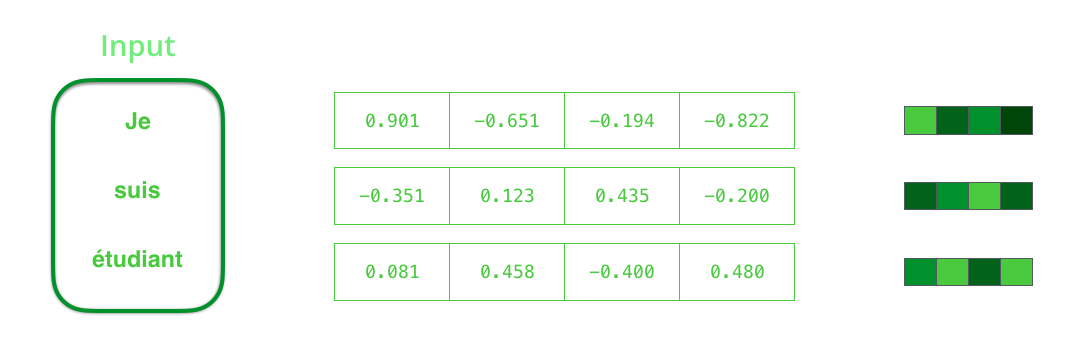
\includegraphics[width=0.8\textwidth]{example_word_embedding.png}
\caption{Example Word Embeddings. From \emph{Visualizing Neural Machine Translation Mechanics of Seq2Seq Models with Attention}, by Jay Alammar, 2018. \url{http://jalammar.github.io/visualizing-neural-machine-translation-mechanics-of-seq2seq-models-with-attention/}. Copyright 2018 by Jay Alammar.}
\end{figure}

According to Rudolph et al. (2016), "each term in a vocabulary is associated with two latent vectors, an \emph{embedding} and a \emph{context vector}. These two types of vectors govern conditional probabilities that relate each word to its surrounding context." 
Rudolph and Blei (2017) note that a word embedding uses vector representations to parameterize the conditional probabilities of words in a surrounding context. 
In other words, a word's conditional probability combines its \emph{embedding} and \emph{context vectors} of surrounding words, with different methods combining them differently. Subsequently, word embeddings are fitted to given text data by maximizing the conditional probabilities of observed text (Rudolph et al. 2017). 

\subsection{Static Embeddings vs. Contextual Embeddings}

\subsubsection{What is Polysemy?}

Polysemy means that a word can have multiple, distinct meanings. The distributional hypothesis in NLP states that meaning depends on context, and words occurring in the same contexts have similar meaning (Wiedemann et al. 2019). 

\subsubsection{The Problem With Static Embeddings: A Context-Free Representation}

Classic word vectors, also called static embeddings, represent words in a low-dimensional continuous space in a static way: this means each word has a single word vector representation regardless of its context (Ethayarajh, 2019). Skip-gram (Mikolov et al., 2013a) and GloVe (Pennington et al., 2014) are well-known algorithms for producing these "context-independent representations," as Peters et al. (2018) calls them, due to the fact that their word embedding matrix, inputted to a neural network representation, is trained to use co-occurring information in text, rather than using dynamic computation offered by language models (Batista, 2018). Although still able to capture latent syntactic and semantic meaning by training over large corpora, static embeddings by definition create a single vector representation per word, so all senses of a polysemous word are collapsed within a single representation (Ethayarajh, 2019). 

\subsubsection{A Better Solution: Contextual Embeddings To Capture Polysemy}

A contextual word embedding (CWE) is

Recent efforts to capture polysemy for word embeddings cast aside the idea of using a fixed word sense inventory. This allows contextual embeddings to "not only create one vector representation for each [word] type in the vocabulary" but to also create separate vectors for each token in a surrounding context. Indeed, experiments show that contextual embeddings can capture word senses successfully (Wiedemann et al., 2019). Wiedemann concludes that this allows for a more realistic model of natural language; contextual embeddings have proven their superiority over static embeddings for many NLP tasks such as text classification (Zampieri et al., 2019) and sequence tagging (Akbig et al., 2018). Although contextualization models such as BERT, ELMo, ERNIE 2.0, and Transformer differ widely, modeling "sentence or context-level semantics together with word-level semantics proved to be a powerful innovation" in the NLP world (Wiedemann et al., 2019). 



----------------


\subsection{Word Embedding Representations: Count-Based vs. Context-Based}

LILIAN WENG: https://hyp.is/dKRaygVnEeqRaI-_7zzFtQ/lilianweng.github.io/lil-log/2017/10/15/learning-word-embedding.html
"There are two main approaches for learning word embedding, both relying on the contextual knowledge.

Count-based: The first one is unsupervised, based on matrix factorization of a global word co-occurrence matrix. Raw co-occurrence counts do not work well, so we want to do smart things on top.
Context-based: The second approach is supervised. Given a local context, we want to design a model to predict the target words and in the meantime, this model learns the efficient word embedding representation."


One way to convert human text into machine-interpretable data is to use a one-hot encoding. Essentially, each distinct word stands for one dimension of the resulting vector a




\subsection{How Word Embeddings are Used}

To complete NLP tasks, NLP models usually choose to use probability as a measure to evaluate a language model. 

Word embeddings are trained as parameters to optimize a generic task-independent objective function. 

Word embeddings are generally fed as vector parameters into a neural network language model. Each row of a word embedding matrix corresponds to a word in the vocabulary, which consists of unique tokens from a corpus. 

The word embedding matrix corresponds to the weights of the neural network, which are trained to minimize an objective or loss function by backpropagating gradients over the neural network. 

Alternatively, we can view this loss function as maximizing the conditional probabilities of words. The conditional probability of a word combines its embedding and the context vectors of its surrounding words. Different language models combine them differently. 

In this way, distributional semantics arises as word embeddings learn to represent context via proximity of related words.  
